\section{Kamma and Natural Decisive Support}

Here is an appropriate joke for the seventh lesson of this Practical Abhidhamma Course: Welcome to the kamma café; there are no menus, you will be served what you deserve. This lesson focuses on kamma and natural decisive support.\footnote{The Pāḷi word for “natural decisive support” is \textit{pakatūpanissaya}.} You are probably familiar with term “kamma,” but may have never heard of “natural decisive support.” Though it may sound like the name of a healthcare product, natural decisive support is actually how the mind is impacted by defilements, \textit{pārami},\footnote{\textit{Pārami} are “perfections,” the 10 qualities leading to Buddhahood: generosity (\textit{dāna}), morality (\textit{sīla}), renunciation (\textit{nekkhamma}), \textbf{Understanding} (\textit{paññā}), \textbf{Energy} (\textit{viriya}), patience (\textit{khanti}), truthfulness (\textit{sacca}), resolution (\textit{adhiṭṭhāna}), loving-kindness (\textit{mettā}) and \textbf{Equanimity} (\textit{upekkhā}). The list of \textit{pārami} is from the Commentary, not from the Suttas (though each of the qualities are found in the Suttas).} accumulations, habits, vows, tendencies, the environment, and recent events.

\subsection*{Penetrative Sutta (AN 6.63)}

\begin{figure}[H]
\begin{quotation}
It is volition (\textit{cetanā}) that I call kamma. For having willed, one acts by body, speech or mind.
\end{quotation}
\caption{Extract of Penetrative Sutta (AN 6.63) that defines kamma.}
\label{fig:AN6_63}
\end{figure}

Let's start with a discussion of kamma. 

In the Penetrative Sutta,\footnote{AN 6.63: \url{http://www.accesstoinsight.org/tipitaka/an/an06/an06.063.than.html\#part-5}} the Buddha defined kamma: “It is \textbf{Volition} (\textit{cetanā}) that I call kamma. For having willed, one acts by body speech or mind.” As mentioned in the lesson on Mental Factors, \textit{cetanā} is translated as either “volition” or “intention.”

The Buddha’s teachings on kamma were revolutionary for the time. In the \textit{Vedas}, the word “kamma” meant ritual action\footnote{The \textit{Vedas} placed considerable emphasis on ritual animal sacrifices.} and had no ethical implications. In the \textit{Upaniṣads}, which slightly pre-date the Buddha, the word “kamma” started to take on an ethical meaning. Many of the Buddha’s contemporaries believed that the ethical quality of kamma was determined by actions, so there was a strong belief that rites and rituals contributed to spiritual development.\footnote{\textbf{Attachment} to rites and rituals (\textit{sīlabbataparāmāsa}) is a fetter (something that binds one to \textit{Saṃsāra}) that is uprooted by the Sotāpanna.} According to Buddhism, kamma arises from the intention behind thought, the intention behind speech and the intention behind action.\footnote{The triad “thought, speech and action,” commonly found in the Suttas, is absent from the \textit{Vedas} and \textit{Upaniṣads} of the time. “Good Thoughts, Good Words, Good Deeds” is a basic maxim of Zoroastrianism (\url{http://en.wikipedia.org/wiki/Zoroastrianism}), suggesting a possible link with Buddhism. (see\\
\url{http://www.academia.edu/1327850/Possible_Iranian_Origins_for_Sakyas_and_Aspects_of_Buddhism}).}

\pagebreak

This shift in focus from action to intention has important implications. For example, if you accidentally step on an insect there is no intention to kill and therefore no kamma of killing. Also, speaking or acting with strong \textbf{Volition} creates much weightier kamma than speaking or acting with weak \textbf{Volition}. The Theravāda view is that wholesome kamma does not arise from ritual action such as taking refuges or precepts; wholesome kamma arises from the intention in the mind while taking refuges or precepts.\footnote{The Suttas do not contain any rituals for laypeople; today’s lay rituals, such as taking refuges and precepts, were originally intended for monastics. The taking of refuges was a request for ordination as a monk (see Vinaya Volume 4, page 30) and the structure of the five precepts is taken from the Vinaya. The wording used to take the five precepts is first found in the Abhidhamma (see \textit{Vibhaṅga}, page 376). Most non-Theravāda schools of Buddhism place greater emphasis on rituals.}

A “Guidelines for new Buddhists” book written 900 years ago says, “If you don’t know the precepts in Pāḷi, say them in your own language. You can recite them individually or just say, ‘I undertake the [precepts] prescribed by the Buddha.’”\footnote{“The Ornament of Lay Followers” (\textit{Upāsakajanālaṅkāra}), page 93.} This shows that according to Buddhism, the actual words used are not a critical factor,\footnote{The Buddha said that the Dhamma should be learned in one’s own dialect (see Vinaya Volume 5, page 194). This is in contrast with the \textit{Vedas} which had to be recited in proper Sanskrit to be effective. So why does Pāḷi play such an important role in the Theravāda tradition? In my opinion, even a superficial understanding of Pāḷi significantly deepens one’s understanding of the Suttas.} but rather it is what is in your heart, the underlying \textbf{Volition}, that is important.

The Buddha disagreed with his contemporaries on the effects of kamma. The Buddha criticized those who believed that all kamma had to be experienced, saying that this was fatalistic, would lead to inaction and lack of moral responsibility.\footnote{AN 3.61: \url{http://www.accesstoinsight.org/tipitaka/an/an03/an03.061.than.html}} For example, if one kills because of past kamma, how can one be held morally responsible? 

The Buddha also criticized those who believed that everything experienced was the result of past kamma and therefore, one should “burn through one’s past kamma.”\footnote{MN 101: \url{http://www.accesstoinsight.org/tipitaka/mn/mn.101.than.html}. This view is attributed to followers of Nigaṇṭha Nātaputta, also known as Mahāvīra (\url{http://en.wikipedia.org/wiki/Mahavira}). These are the Jains (\url{http://en.wikipedia.org/wiki/Jainism}).} He explained that past kamma is only one of the factors impacting what we experience, and that the view that new kamma was to be avoided would lead to inaction.\footnote{SN 36.21: \url{http://www.accesstoinsight.org/tipitaka/sn/sn36/sn36.021.than.html}}

According to Buddhism, kamma is an impersonal law of nature; a natural law like gravity or magnetism.\footnote{The Commentary refers to this “natural, fixed law of kamma” as \textit{kamma-niyāma}. Other natural, fixed laws defined in the Commentary cover temperature, seasons and physical events (\textit{utu-niyāma}), plant life (\textit{bīja-niyāma}), the sequence of Mind Moments (\textit{citta-niyāma}) and certain events connected with the Dhamma (\textit{dhamma-niyāma}) such as events occurring in the lives of Buddhas.} In fact, the Buddha compared the law of kamma with the law of gravity.\footnote{SN 42.6: \url{http://www.accesstoinsight.org/tipitaka/sn/sn42/sn42.006.than.html}}

It is common to hear Buddhists who are facing difficulties say, “It is my kamma.” This statement is wrong in two ways. First, kamma is created and one experiences the results of kamma, so rather than saying “It is my kamma,” the correct phrase would be, “It is my kamma-result.”\footnote{The Pāḷi word for “kamma-result” is \textit{vipāka}.} Secondly, and more importantly, “It is my kamma” is a fatalistic attitude and does not take into account the conditions other than kamma that can lead to a result. Everything arises because of multiple conditions.\footnote{Visuddhimagga XVII.105 (see Footnote 2 for link).} 

\pagebreak

For example, you cannot blame sickness just on kamma-result. Kamma-result may play a role in a sickness arising, but the environment, clean or disease-infested, plays a role as well. We can increase our chances of avoiding sickness by changing our environment.

Imagine that I go into a room and turn on the light. To say that the light went on because I pressed the light switch is only partially correct. There were also many supporting conditions that were created in the past. A power plant was built, transmission lines erected, the building was wired and somebody installed a light bulb. All of this supporting infrastructure was needed for the action of pressing the light switch to result in the light going on. Similarly, all that supporting infrastructure created in the past still needs the effort in the present of me pressing the light switch to turn on the light. My past kamma can find an opportunity to ripen if suitable effort is made in the present.

I visualize myself as being surrounded by a cloud of countless wholesome and unwholesome “kamma-seeds,” waiting for suitable conditions to ripen.\footnote{This Sutta (AN 3.33) uses the image of “kamma-seeds” and also explains that Arahat do not create new kamma: \url{http://www.accesstoinsight.org/tipitaka/an/an03/an03.033.than.html}} Living in a wholesome environment with many wholesome influences and keeping my precepts creates conditions for wholesome kamma-seeds to ripen. Similarly, if I were to live in an unwholesome environment with many unwholesome influences and ignore my precepts, this would create conditions for unwholesome kamma-seeds to ripen.\footnote{This visualization of “kamma-seeds” should not be taken too literally. The Yogācāra school of Buddhism (\url{http://en.wikipedia.org/wiki/Yogacara}) introduced the idea of a “storehouse consciousness” (Sanskrit: \textit{ālayavijñāna}) to store kammic potential (\url{http://en.wikipedia.org/wiki/Eight_Consciousnesses}). The Theravāda school rejected this doctrine as an attempt to create a Self.}

\subsection*{Shorter Exposition of Kamma Sutta (MN 135)}

\begin{figure}[H]
\begin{quotation}
Subha: “One meets with short-lived and long-lived people, sick and healthy people, ugly and beautiful people, insignificant and influential people, poor and rich people, low-born and high-born people, stupid and wise people. What is the reason, what is the condition, why superiority and inferiority are met with among human beings?”

Buddha: “Beings are owners of their kamma, heirs of their kamma; they originate from their kamma, are bound to their kamma and have their kamma as their refuge.”

A person who kills is reborn in an unhappy destination, or if reborn as human they have a short life. A person who refrains from killing is reborn as a god, or if reborn as a human they have a long life.

… injures others \textrightarrow \hspace{1mm} sickly

… angry \textrightarrow \hspace{1mm} ugly

… envious \textrightarrow \hspace{1mm} insignificant

… stingy \textrightarrow \hspace{1mm} poor

… arrogant \textrightarrow \hspace{1mm} low-born

… does not reflect on spiritual matters \textrightarrow \hspace{1mm} stupid
\end{quotation}
\caption{Extract of Shorter Exposition of Kamma Sutta (MN 135).}
\label{fig:MN135}
\end{figure}

Let’s now move on to the extract from the “Shorter Exposition of Kamma Sutta” shown in Figure \ref{fig:MN135}.\footnote{MN 135: \url{http://www.accesstoinsight.org/tipitaka/mn/mn.135.than.html}} Before discussing the contents of this Sutta, here is the background story as recorded in the Commentary.\footnote{Summarized from Bodhi Leaves 128, published by the Buddhist Publication Society: \url{http://www.bps.lk/olib/bl/bl128.pdf}}

Todeyya was a very rich Brahmin who was also very stingy; he refused to support virtuous people and tried to prevent others from giving alms.\footnote{Todeyya recited the \textit{Vedas} at ceremonies officiated by King Pasenadi. King Pasenadi was very generous to Todeyya, making Todeyya very rich and very proud.} When Todeyya died, his only son Subha inherited Todeyya’s mansion and wealth. Todeyya was so attached to his mansion that he was reborn as a watchdog, living in the mansion.

One day, the Buddha was on alms round and stopped in front of the mansion. The watchdog started barking and the Buddha gently said, “Todeyya, not only now but also in your previous birth did you treat me in this way. This is why you were born as a dog.” The dog immediately ran to hide in the back of the house. When Subha returned later, he was surprised that the dog did not rush out to greet him. The servants told Subha what the Buddha had said to the dog and Subha was furious. Brahmins are very proud people and dogs were considered to be disgusting animals, so it was a serious insult to say that Todeyya had been reborn as a dog.

Subha went to scold the Buddha. The Buddha calmed Subha’s mind and said, “Is it not true that your father buried some treasure somewhere on your property?” Subha confirmed that this was true. The Buddha said, “Go home and feed the dog well. Once the dog has fallen asleep, whisper in its ear, ‘Father, where is the treasure?’ When the dog takes you to the treasure, this will prove that the dog was your father.” Subha was happy. If the dog did not reveal the treasure, Subha could discredit the Buddha. If the dog did reveal the treasure, Subha would be much richer. Of course, the dog led Subha to the treasure. This caused Subha to wonder about the workings of kamma and Subha decided to approach the Buddha for clarification.

At the beginning of the Sutta, Subha approaches the Buddha and says, “One meets with short-lived and long-lived people, sick and healthy people, ugly and beautiful people, insignificant and influential people, poor and rich people, low-born and high-born people, stupid and wise people. What is the reason, what is the condition, why superiority and inferiority are met with among human beings?”

The Buddha gave a short reply, “Beings are owners of their kamma, heirs of their kamma; they originate from their kamma, are bound to their kamma and have their kamma as their refuge.” On another occasion, the Buddha recommended that both laypeople and monks should often reflect on these same words.\footnote{AN 5.57: \url{http://www.accesstoinsight.org/tipitaka/an/an05/an05.057.than.html}}

“Beings are owners of their kamma” means that whatever kamma we have is our only true possession; we don’t bring anything into this world except our kamma and we can’t take anything out of this world except our kamma. “Beings are the heirs of their kamma” means that we inherit our kamma from our past existence. “Beings originate from their kamma” means that we are born because of kamma. “Beings are bound to their kamma” means that we are never separated from our kamma. “Beings have kamma as their refuge” means that we must rely on our kamma for future rebirths.

\pagebreak

Subha said that he did not understand this short reply and asked for a more detailed explanation. You may wonder why the Buddha would give an answer that would confuse the questioner. The reason was that being a Brahmin, Subha was very proud, and the Buddha needed to reduce Subha’s \textbf{Conceit} a bit before Subha would be ready to accept the Buddha’s teachings.\footnote{The Buddha frequently used this approach when replying to questions from Brahmins.}

The Buddha started his more detailed analysis of kamma with, “A person who kills is reborn in an unhappy destination, or if reborn as human they have a short life.” 

An unhappy destination would include the Hell realm, the animal realm, the \textit{Peta} realm or the \textit{Asura} realm. Killing can never lead to a human rebirth, so the second part of the sentence means, “If some other wholesome kamma causes rebirth as a human, then the unwholesome kamma associated with killing from the previous existence can reduce the lifespan in the human existence.” In other words, the unwholesome kamma of killing can either determine rebirth or can arise during a future existence. If the unwholesome kamma of killing arises during a future human existence, it will shorten the lifespan.

The Buddha continued his explanation with, “A person who refrains from killing is reborn as a god, or if reborn as a human they have a long life.” 

Since kamma is driven by \textbf{Volition}, “refraining from killing” cannot be passive, it has to be active, with intention. You can’t stay in bed all day and then say, “I didn’t kill today, I didn’t go hunting, so I deserve to go to heaven.” An example of actively refraining from killing is blowing at a mosquito when it lands on your arm rather than swatting it. Actively refraining from killing, in spite of an opportunity, can create kamma that conditions rebirth in the \textit{Deva} realm. On the other hand, if some other wholesome kamma conditions rebirth as a human, actively refraining from killing in a past existence can extend the lifespan in that human existence.

If a person injures others, the unwholesome kamma created can lead to rebirth in an unhappy destination. Alternatively, if some other wholesome kamma leads to rebirth as a human being, the unwholesome kamma created in the past life by injuring others will cause the human being to be sickly. 

If a person actively refrains from injuring others, puts \textbf{Compassion} into action, the wholesome kamma created can lead to rebirth as a \textit{Deva}. Alternatively, if some other wholesome kamma leads to rebirth as a human being, the wholesome kamma created by \textbf{Compassion} in the past existence will cause the human being to be healthy.

Similarly, an angry person may be reborn as ugly while loving-kindness leads to rebirth with beauty. An envious person may be reborn as insignificant while a contented person may be reborn as influential. A stingy person may be reborn as poor while a generous person may be reborn as rich. An arrogant person may be reborn as low-born while a humble person may be reborn as being well respected.\footnote{The Sutta says, “high born,” which probably referred to caste at the time of the Buddha. I chose the term “well respected” to be relevant in today’s non-Indian society.} A person who does not reflect on spiritual matters may be reborn as stupid while a person who is spiritually inclined may be reborn as wise.

Regarding the last point, the Sutta actually says “a person who does not ask questions from a recluse or Brahmin may be reborn as stupid.” Some Dhamma speakers joke that if you don’t ask questions after the Dhamma talk, you may be reborn as stupid. In my opinion, the fact that you have made the effort to folow these lessons will create good kamma for you, so Congratulations! \smiley 

\pagebreak

\subsection*{Kamma Results Sutta (AN 8.40)}

\begin{figure}[H]
\begin{quotation}
A person who steals is reborn in an unhappy destination, or if reborn as human they will tend to lose wealth.

… commits sexual misconduct \textrightarrow \hspace{1mm} tend to face ill-will and rivalry

… lies \textrightarrow \hspace{1mm} tend to face false accusations

… slanders \textrightarrow \hspace{1mm} tend to be divided from their friends

… uses harsh speech \textrightarrow \hspace{1mm} tend to hear disagreeable sounds

… indulges in idle talk \textrightarrow \hspace{1mm} tend to have others distrusting one’s words

… indulges in intoxicants \textrightarrow \hspace{1mm} tend to mental derangement
\end{quotation}
\caption{Extract of Kamma Results Sutta (AN 8.40).}
\label{fig:AN8_40}
\end{figure}

The Kamma Results Sutta has a similar structure to the Shorter Exposition of Kamma Sutta and covers additional results of kamma.\footnote{AN 8.40: \url{http://www.accesstoinsight.org/tipitaka/an/an08/an08.040.than.html}} The Kamma Results Sutta only mentions the negative consequences, but I think that we can extrapolate the positive consequences of actively avoiding unwholesome kamma based on the “Shorter Exposition of Kamma Sutta.”

Since there is a “Shorter Exposition of Kamma Sutta,” it should come as no surprise that there is a “Greater Exposition of Kamma Sutta.”\footnote{MN 136: \url{http://www.accesstoinsight.org/tipitaka/mn/mn.136.than.html}} The main message of this Sutta is that people who have committed wholesome deeds may end up with either an unfortunate rebirth or with a fortunate rebirth. Similarly, people who have committed unwholesome deeds may end up with either an unfortunate rebirth or with a fortunate rebirth. There is often an element of randomness in a single rebirth. \textit{Saṃsāra} involves many rebirths, and past kamma is always looking for suitable conditions to ripen.

\subsection*{Salt Crystal Sutta (AN 3.99)}

\begin{figure}[H]
\begin{quotation}
There is the case where a trifling evil deed done by a certain individual takes him to Hell. There is the case where the very same sort of trifling deed done by another individual is experienced in the here-and-now, and for the most part barely appears for a moment.

There is an individual who is undeveloped in contemplating the body, undeveloped in virtue, undeveloped in mind, undeveloped in discernment: restricted, small-hearted, dwelling with suffering. A trifling evil deed done by this sort of individual takes him to Hell.

There is an individual who is developed in contemplating the body, developed in virtue, developed in mind, developed in discernment: unrestricted, large-hearted, dwelling with the immeasurable. A trifling evil deed done by this sort of individual is experienced in the here-and-now, and for the most part barely appears for a moment. 

A salt crystal in a small cup makes the water undrinkable and a salt crystal in the River Ganges has no effect. In the same way a trifling evil deed takes one individual to Hell and the same sort of trifling deed done by the other individual is experienced in the here-and-now, and for the most part barely appears for a moment.
\end{quotation}
\caption{Extract of Salt Crystal Sutta (AN 3.99).}
\label{fig:AN3_99}
\end{figure}

The Buddha warned that trying to understand the detailed workings of kamma could drive you crazy,\footnote{AN 4.77: \url{http://www.accesstoinsight.org/tipitaka/an/an04/an04.077.than.html}} so let’s not spend time on these details. The detailed workings of kamma are impossible to fathom, but the Salt Crystal Sutta gives us a general strategy on how to work with kamma. Let me start by reading an extract from the Salt Crystal Sutta from Figure \ref{fig:AN3_99}.

There is the case where a trifling evil deed done by a certain individual takes him to Hell. There is the case where the very same sort of trifling deed done by another individual is experienced in the here-and-now, and for the most part barely appears for a moment.

Before going further, I should explain what the Budddha meant by the result of kamma being experienced in the here-and-now, usually barely appearing for a moment. If kamma plays a role at the time of rebirth, the effect lasts a long time (an entire existence). When kamma ripens during a lifetime, it is usually as a moment of physical pain or as a moment of physical pleasure. Of course, physical pain is often both preceded and succeeded by Mind Moments with mental unpleasant feeling, but Mind Moments with mental unpleasant feeling are not the result of kamma. I will now continue reading the extract from the Sutta.

There is an individual who is undeveloped in contemplating the body, undeveloped in virtue, undeveloped in mind, undeveloped in discernment: restricted, small-hearted, dwelling with suffering. A trifling evil deed done by this sort of individual takes him to Hell.

\pagebreak

There is an individual who is developed in contemplating the body, developed in virtue, developed in mind, developed in discernment: unrestricted, large-hearted, dwelling with the immeasurable.\footnote{“Dwelling with the immeasurable” means the mind is absorbed in loving-kindness (\textit{mettā}), \textbf{Compassion} (\textit{karuṇā}), \textbf{Sympathetic joy} (\textit{muditā}) or \textbf{Equanimity} (\textit{upekkhā}). These states are called ``immeasurable" (\textit{appamañña}), sometimes translated as ``boundless", because they are applied to all beings. They are also called the ``Divine Abodes" (\textit{brahma-vihāra}). See: \url{http://www.accesstoinsight.org/lib/authors/nyanaponika/wheel006.html}} A trifling evil deed done by this sort of individual is experienced in the here-and-now, and for the most part barely appears for a moment.

A salt crystal in a small cup makes the water undrinkable, and a salt crystal in the River Ganges has no effect. In the same way, a trifling evil deed takes one individual to Hell, and the same sort of trifling deed done by the other individual is experienced in the here-and-now, and for the most part barely appears for a moment.

In other words, if unwholesome kamma ripens, it will always result in unwholesome kamma-result, but the intensity and duration of the result may be very different from the weightiness of the original. An unwholesome kamma-result may still arise, but present conditions may “water down the effect” of unwholesome kamma-result. Present conditions such as living in a wholesome environment with many wholesome influences and keeping precepts will naturally allow past wholesome kamma to ripen. Such wholesome present conditions may not stop past unwholesome kamma from ripening, but if it does ripen, the result will be experienced barely for a moment.

Returning to the example of turning on the light using the light switch, it may seem that a relatively small effort of pressing the light switch had a relatively large effect of lighting up the entire room. But it is actually more complicated than that when one considers the infrastructure that was needed. In summary, don’t worry so much about what kamma was created in the past, focus on creating wholesome present conditions.

%\pagebreak

\subsection*{Angulimāla Sutta (MN 86)}

\begin{figure}[h]
\centering
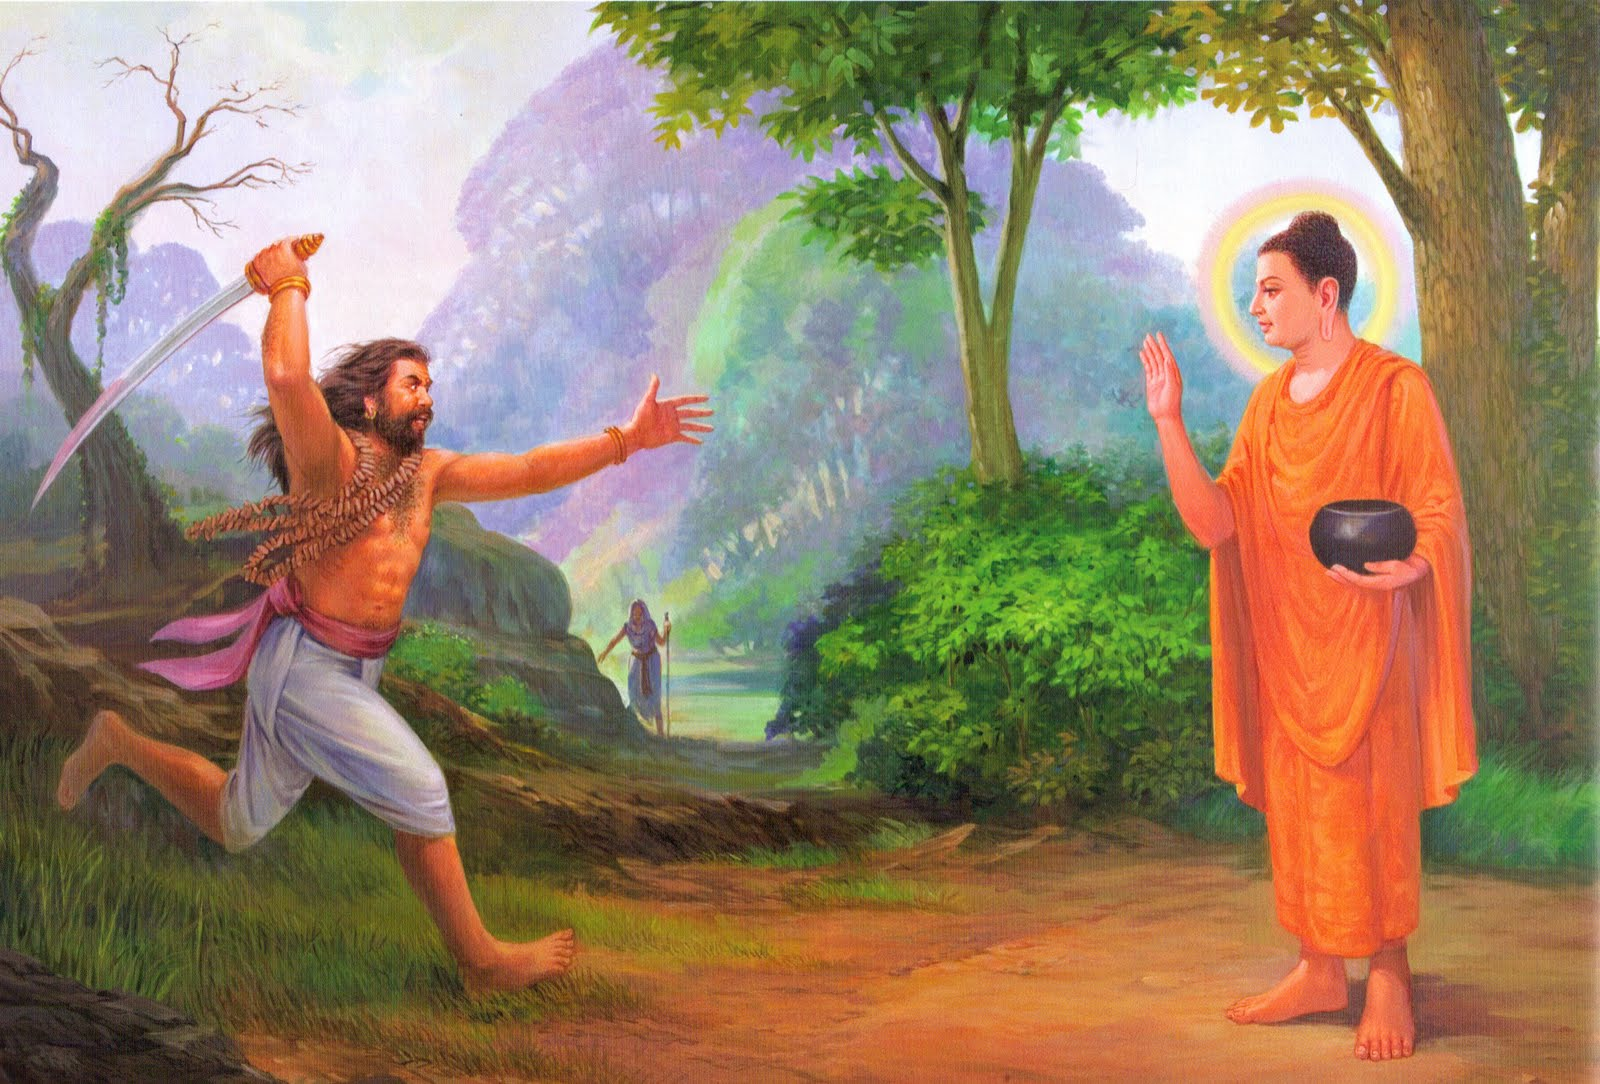
\includegraphics[width=0.8\linewidth]{./Diagrams/angulimala}
\caption{The story of Angulimāla, the killer tamed by the Buddha, is popular in Buddhist countries.}
\label{fig:angulimala}
\end{figure}

The Angulimāla Sutta gives an example of how past unwholesome kamma may be “watered down.”\footnote{MN 86: \url{http://www.accesstoinsight.org/tipitaka/mn/mn.086.than.html}} Before meeting the Buddha, Angulimāla was a serial killer. The story of how he was converted into an Arahat is also found in the Commentary.\footnote{\url{http://www.tipitaka.net/tipitaka/dhp/verseload.php?verse=173}} The following incident happened after Angulimāla had become an Arahat.

\begin{figure}[H]
\begin{quotation}
Then Venerable Angulimāla, early in the morning, having put on his robes and carrying his outer robe and bowl, went into Sāvatthī for alms. Now at that time a clod thrown by one person hit Venerable Angulimāla on the body, a stone thrown by another person hit him on the body, and a potsherd thrown by still another person hit him on the body. So Venerable Angulimāla – his head broken open and dripping with blood, his bowl broken, and his outer robe ripped to shreds – went to the Blessed One. The Blessed One saw him coming from afar and on seeing him said to him: “Bear with it, brahmin! Bear with it! The fruit of the kamma that would have burned you in Hell for many years, many hundreds of years, many thousands of years, you are now experiencing in the here-and-now!”
\end{quotation}
\caption{Extract of Angulimāla Sutta (MN 86).}
\label{fig:MN86}
\end{figure}

Obviously, Angulimāla had accumulated considerable unwholesome kamma from killing so many people before becoming a monk. Yet because of Angulimāla’s current condition of being an Arahat, the kammic result was reduced to some cuts and bruises. I think all of us have done some things in the past of which we are not proud. We should focus on creating wholesome conditions in the present; wholesome environment with many wholesome influences and keeping our precepts. And if by chance some past unwholesome kamma finds an opportunity to ripen, remember the Buddha’s words, “Bear with it!”

\subsection*{Completed Kamma}

\begin{figure}[H]

\begin{quote}

\tablesubheader{Killing}: \ding{172} A living being \ding{173} Knowledge \ding{174} Intention \ding{175} Effort \ding{176} Death

\tablesubheader{Stealing}: \ding{172} Property \ding{173} Knowledge \ding{174} Intention \ding{175} Effort \ding{176} Removal

\tablesubheader{Sexual Misconduct}: \ding{172} Forbidden partner (married / under guardianship) \ding{173} Intention \ding{174} Effort \ding{175} Acceptance

\tablesubheader{Lying}: \ding{172} Untrue thing \ding{173} Intention \ding{174} Effort \ding{175} Communication

\tablesubheader{Slander}: \ding{172} People to be separated \ding{173} Intention \ding{174} Effort \ding{175} Separation

\tablesubheader{Harsh Speech}: \ding{172} Person \ding{173} Intention \ding{174} Effort

\tablesubheader{Idle Talk}: \ding{172} Inclination toward idle talk \ding{173} Effort \ding{174} Others accept 

\tablesubheader{Covetousness}: \ding{172} Property \ding{173} Thought of “I wish it were mine”

\tablesubheader{Ill Will}: \ding{172} Another person \ding{173} Thought of “I hope that the other person is destroyed”

\tablesubheader{Wrong view}: \ding{172} Ideas of “no kamma”/“no cause”/“no cause and no result” \ding{173} Manifestation

\end{quote}

\caption{Conditions required to make kamma “completed.”}
\label{fig:Completed}
\end{figure}

Let’s now proceed to the topic of “Completed Kamma.” As mentioned in the previous lesson, “Completed Kamma” is sufficiently weighty to condition rebirth. For example, the kamma created when I enjoy my coffee is not weighty enough to condition rebirth. \textbf{Attachment} to my coffee still creates unwholesome kamma, but not the rebirth-linking kind of kamma.

The Buddha listed ten unwholesome actions that can cause rebirth in a woeful plane: killing, stealing, sexual misconduct, lying, slander, harsh speech, idle talk, coveting, ill will and \textbf{Wrong view}.\footnote{MN 41: \url{http://www.accesstoinsight.org/tipitaka/mn/mn.041.nymo.html\#unwholesome10}} According to the Commentary, for an unwholesome action to condition rebirth in a woeful plane, certain conditions must be met, and when all of these conditions are met, it is considered to be “completed kamma.” The Commentary also identifies the factors that, in addition to \textbf{Volition}, impact the weight of the kamma produced.\footnote{“The Expositor” (\textit{Atthasālinī}), pages 128--134.}

For killing, the required factors are: a living being (human or animal), knowledge that the being exists, intention to kill, effort to kill and consequential death. Killing a virtuous person is weightier than killing an immoral person, killing a human is weightier than killing an animal, killing a domesticated animal is weightier than killing a wild animal, killing a large animal is weightier than killing a small animal.\footnote{It requires a lot more effort (and thereby more intention) to kill a large animal as compared to killing a small animal such as a mosquito.}

The Commentary mentions\footnote{\url{http://www.tipitaka.net/tipitaka/dhp/verseload.php?verse=001}} a blind monk who inadvertently stepped on insects while doing walking meditation. The Buddha explained that the monk had done nothing wrong because there was no awareness of the existence of the insects and no intention to kill. 

\pagebreak

Buying meat at the grocery store or ordering meat from the menu of a restaurant are not killing, because there is no intention to have an animal killed specifically for you. On the other hand, it is considered killing if you order fresh seafood at a restaurant that keeps live seafood in tanks. The Buddha did allow monks to eat meat and fish, as long as the monk does not suspect that the meat or fish was killed for the purpose of feeding monks.\footnote{See Vinaya Volume 4, page 325. Also on page 298: Certain types of meat were not allowed under any circumstances: humans, horses and elephants (considered too noble to eat), dogs (considered to be too disgusting to eat), snakes, lions, tigers, leopards, bears and hyenas (there was a belief that eating one of these predators would give off a smell causing similar predators to attack the monk).}

There is a story in the Commentary of a female Sotāpanna who prepared weapons for her husband who was a hunter. The Buddha explained that she did not break the precept of avoiding killing because she was only preparing things for her husband.\footnote{\url{http://www.tipitaka.net/tipitaka/dhp/verseload.php?verse=124}}

Both the judge who issues a death sentence and the executioner who performs the act are guilty of killing. Suicide, euthanasia, mercy killing and abortion are all considered to be killing. There is no fault in killing plants, bacteria or germs because they do not have consciousness and are therefore not considered to be “living beings.”\footnote{Monks should not cut down plants (see Vinaya Volume 2, page 226 \url{http://www.accesstoinsight.org/tipitaka/vin/sv/bhikkhu-pati.html\#pc-11}); this is to avoid causing inconvenience to any \textit{Deva} who may be living there.}

For stealing, the required factors are: another’s property, knowledge that it is another’s property, intention to steal, effort to steal and removal of the property. Stealing from a virtuous person is weightier than stealing from an immoral person. Stealing a valuable object is weightier than stealing a worthless object.

The Commentary mentions that forgery or using false weights when conducting business is considered to be stealing. Personal use of the office photocopier or making personal phone calls during office hours is also stealing. Buying something in another country to avoid paying import duties in your home country is also stealing.\footnote{This is stealing from the government by illegally avoiding paying import duties. Buying things at the Duty Free shop is legally avoiding paying import duties, so this is not considered to be stealing.}

For sexual misconduct, the required factors are a woman who is forbidden, lustful intention, engaging in sexual intercourse and acceptance of the union. Sexual misconduct with a virtuous woman is weightier than with an immoral woman. A woman is forbidden if she is married, engaged, under the guardianship of a family member, a convict or a nun.

Adultery is sexual misconduct. A rapist is guilty of sexual misconduct but the victim of rape is not guilty because there was no acceptance of the union. Assuming that the factors are not met, the definition of sexual misconduct does not prohibit premarital sex,\footnote{At the time of the Buddha, people were married in their early teens, so premarital sex was not an issue.} homosexuality\footnote{The Suttas are silent on the subject of homosexuality among laypeople. Any form of sexual activity is prohibited for monastics.} or prostitution.\footnote{Associating with prostitutes is a cause of downfall (see Sn 1.6: \url{http://www.accesstoinsight.org/tipitaka/kn/snp/snp.1.06.nara.html}).}

For lying, the required factors are an untrue thing, intention to deceive, effort to deceive and communication of the untruth. The weightiness depends on the amount of welfare destroyed by the lie. Telling “white lies” to get children to behave, to close a business deal or insincere flattery are all lying. If an accountant conceals financial irregularities under instruction from their boss, both are lying.

\pagebreak

For slander, the required factors are people to be separated, intention to separate them, effort to separate them and separation. Slandering a virtuous person is weightier than slandering an immoral person.

For harsh speech, the required factors are a person to be abused, an angry thought and the abuse. Abusing a virtuous person is weightier than abusing an immoral person. Reminds me of a joke: before you criticize someone, walk a mile in his shoes. That way, if he gets angry, he’ll be a mile away and barefoot.

For idle talk, the required factors are an inclination toward useless topics of conversation such as politics, fashion or gossip,\footnote{The list of useless topics of conversation (\textit{tiracchānakathā}; literally “animal talk”) is found in AN 10.69 (\url{http://www.accesstoinsight.org/tipitaka/an/an10/an10.069.than.html}): “conversation about kings, robbers, ministers of state, armies, alarms, battles, food and drink, clothing, furniture, garlands, scents, relatives, vehicles, villages, towns, cities, the countryside, women and heroes, the gossip of the street and the well, tales of the dead, tales of diversity, the creation of the world and of the sea, talk of whether things exist or not.”} talking about useless topics and other’s accepting the conversation. Frequent indulgence in idle talk makes the kamma weightier. My personal view is that involvement in politics is not conducive to one’s spiritual development. In fact, monks are not allowed to vote in elections in Myanmar or Thailand.\footnote{Sri Lankan monks can vote and there is a political party led by monks: (\url{http://en.wikipedia.org/wiki/Jathika_Hela_Urumaya}).} Reminds me of a joke: four monks are meditating when a flag stars flapping. The first monk says, “Flag is flapping,” the second monk says, “Wind is flapping,” the third monk says, “Mind is flapping” and the fourth monk says “Mouths are flapping.”

For coveting, the required factors are another’s property and the thought, “I wish it were mine.” Coveting the property of a virtuous person is weightier than coveting the property of an immoral person. Coveting a valuable object is weightier than coveting a worthless object.

For ill will, the required factors are another person and the thought, “I hope that the other person is destroyed.” Harbouring ill will against a virtuous person is weightier than harbouring ill will against an immoral person. Merely disliking another person is not completed kamma unless there is the thought of “I wish that they were dead.”

For \textbf{Wrong view}, the required factor is the arising idea of “there is no kamma,” “there is no cause” or “there is no cause and no result.” Frequent \textbf{Wrong view} makes the kamma weightier. Denying kamma and thinking “there are no consequences” leads to a lack of moral responsibility.

\pagebreak

\subsection*{Classifications of kamma in the Commentary}

\begin{figure}[H]
\begin{quote}
\tablesubheader{By way of function}: \ding{172} Productive kamma \ding{173} Supportive kamma \ding{174} Obstructive kamma \ding{175} Destructive kamma

\tablesubheader{By time of ripening}: \ding{172} Immediately effective kamma \ding{173} Subsequently effective kamma \ding{174} Indefinitely effective kamma \ding{175} Defunct kamma

\tablesubheader{By order of ripening}: \ding{172} Weighty kamma \ding{173} Death proximate kamma \ding{174} Habitual kamma \ding{175} Reserve kamma

\tablesubheader{By place of ripening}: \ding{172} Unwholesome kamma \ding{173} Sense sphere wholesome kamma \ding{174} Fine material sphere kamma \ding{175} Immaterial sphere kamma

\end{quote}

\caption{Classifications of kamma in the Commentary: By way of function, by time of ripening, by order of ripening and by place of ripening.}
\label{fig:Classifications}
\end{figure}

\subsubsection*{Kamma by way of function}

The Commentary defines four types of kamma by way of function; productive kamma, supportive kamma, obstructive kamma and destructive kamma.

At the time of rebirth, productive kamma determines the new realm of existence and the new gender; things that do not change throughout the existence. During existence, productive kamma supports continued life of the body and produces other results.

Supportive and obstructive kamma arise during an existence, not at rebirth. Supportive and obstructive kamma do not produce its own results, but works to extend or diminish the functions of the productive kamma. For example, supportive kamma can extend our lifespan, just like healthy eating and exercise. Obstructive kamma can decrease our lifespan, just like junk food and an unhealthy lifestyle.

Destructive kamma cuts off and replaces the function of productive kamma. For example, destructive kamma can suddenly cut a life short, as in a fatal accident.

When discussing destructive kamma, I am often asked, “What is the role of kamma when there is an airplane crash and everybody on board dies?” The cause of the crash had nothing to do with kamma. Earthquakes, fires and airplane crashes are not caused by kamma. Kamma works at an individual level. A Sutta explains, “That kamma of yours was not done by your mother, not by your father, not done by your brother, sister, friends and companions, kinsmen and relatives, and not done by the \textit{Devas}. That kamma was done by you yourself, and you yourself will experience its result.”\footnote{MN 130: \url{http://www.accesstoinsight.org/tipitaka/mn/mn.130.than.html\#yama}} All of us, including all the people on the airplane, have had uncountable unwholesome intentions in past lives and in this life. Everybody is carrying with them past kamma that has the potential to arise as destructive kamma when supported by other conditions. So for each of the people on the airplane, the crash was a condition for their individual destructive kamma to arise and cut short their lifespan.

\pagebreak

\subsubsection*{Kamma by time of ripening}

The Commentary classifies kamma according to the time of ripening. As we will discuss during the next lesson on processes, seven identical kamma-creating Mind Moments arise in sequence as part of the sensing process and as part of the thinking process.

The first of the seven kamma-creating Mind Moments is the weakest.\footnote{It is weak because the previous Mind Moment is of a different type.} This creates “immediately effective kamma,” kamma that can ripen only in the current existence. If at the end of the current existence, this kamma has not found conditions to ripen, it becomes “defunct.”

The last of the seven kamma-creating Mind Moments is the second weakest.\footnote{It is weak because the subsequent Mind Moment is of a different type.} This creates “subsequently effective kamma,” kamma that can ripen only in the next existence. If at the end of the next existence, this kamma has not found conditions to ripen, it becomes “defunct.”

The middle five of the kamma-creating Mind Moments are strong.\footnote{They are strong because they are supported by presence of the same kind of Mind Moment both before and after their arising.} These Mind Moments create “indefinitely effective kamma” that can arise any time after the next existence. These kamma never become defunct as long as the round of rebirths continues.

\subsubsection*{Kamma by order of ripening}

The Commentary classifies rebirth-linking kamma according to the order of ripening at the moment of death. There are four classifications of rebirth-linking kamma: weighty kamma, death proximate kamma, habitual kamma and reserve kamma.

Weighty kamma will definitely ripen when death occurs. If one kills one’s mother, kills one’s father, kills an Arahat, wounds a Buddha or maliciously causes a split in the Sangha, then it is guaranteed that the next rebirth will be in Hell. If one maintains a jhāna until the moment of death, rebirth is guaranteed in the fine material plane or the immaterial plane, depending on the level of jhāna.\footnote{Visuddhimagga XIX.15 (see Footnote 2 for link).} 

If one attains jhāna during a retreat and goes back to the world without maintaining it, the jhāna attainment will not qualify as weighty kamma. If one develops the jhāna and later commits one of the five heinous crimes, the good kamma would be obliterated by the evil deed. For example, when Devadatta\footnote{\url{http://en.wikipedia.org/wiki/Devadatta}} wounded the Buddha and caused a split in the Sangha, he lost his psychic powers associated with jhāna and was guaranteed rebirth in Hell.\footnote{Devadatta lost his psychic power in Vinaya Volume 5, page 260 and was guaranteed to be reborn in \textit{Avīci} Hell in Vinaya Volume 5, page 271. Also see story from the Commentary: \url{http://www.tipitaka.net/tipitaka/dhp/verseload.php?verse=017}} If someone were first to commit one of the heinous crimes, they would not be able later to attain jhāna or sainthood because the evil kamma would create an insurmountable obstruction. 

For example, at the end of a discourse to King Ajātasattu, the Buddha said, “If he had not killed his father, the King could have attained sainthood while listening to that discourse.”\footnote{In the Theravāda version of the Sutta (DN 2: \url{http://www.accesstoinsight.org/tipitaka/dn/dn.02.0.than.html\#eye}), even the Buddha could not help King Ajātasattu escape the results of weighty kamma. In the Mahāyāna version of the Sutta, the simple act of meeting the Buddha reduces or eliminates the consequences of the King’s patricide. The concept of kamma evolved over time (see \url{http://blogs.dickinson.edu/buddhistethics/files/2014/01/Jayarava-Karma-final.pdf}).}

\pagebreak

It is highly unlikely that we will commit any of the five heinous deeds or die while in jhāna, so our most likely rebirth-linking kamma will be “death proximate kamma.” This is a strong thought that arises close to the time of death. I was fortunate to be at my mother’s bedside when she passed away. I kept reminding her of the many good things she had done during her life. I wanted her to die with wholesome thoughts. 

There is a story in the Commentary of an executioner who was reborn in heaven because he had just heard the Dhamma.\footnote{\url{http://www.tipitaka.net/tipitaka/dhp/verseload.php?verse=100}} In another story, a virtuous monk was reborn as a flea in his robe because he was attached to the robe.\footnote{\url{http://www.tipitaka.net/tipitaka/dhp/verseload.php?verse=240}} In yet another story, a queen who was a great supporter of the Buddha had an unfortunate rebirth because her last thought was of a single immoral act that she had done.\footnote{\url{http://www.tipitaka.net/tipitaka/dhp/verseload.php?verse=151}} On the surface, it may seem that the executioner, the virtuous monk and the queen were treated unfairly, but they still carried the kammic seeds from their previous deeds which would have an opportunity to arise later.\footnote{Countering the superficial understanding of kamma is one of the themes of MN 137: \url{http://www.accesstoinsight.org/tipitaka/mn/mn.136.than.html}}

If there is no strong “death proximate kamma,” then “habitual kamma” has an opportunity perform the function of rebirth-linking. As its name implies, “habitual kamma” arises from a repetitive action such as regularly meditating or regularly drinking alcohol.

Finally, if there is no weighty kamma, no strong death proximate kamma and no habitual kamma, then some random, reserve kamma can arise. This reserve kamma may even be from a previous life. 

For example, earlier I mentioned the virtuous monk who was reborn as a flea in his robe because of unwholesome “death proximate” kamma. After this monk died, the Buddha instructed the other monks not to touch the robe for seven days. This would ensure that the flea would not get upset, and the flea’s reserve kamma could then allow the flea to be reborn in heaven. 

I also mentioned the queen who had an unfortunate rebirth because of her last thought. When the queen died, the king decided to go to the Buddha to ask about her plane of rebirth. The Buddha distracted the king and he forgot to ask the question so he returned the next day. For seven days the Buddha caused the king to forget his question, but on the eighth day, the queen had been reborn in heaven because of the random kamma of her past good deeds. The Buddha then told the king that the queen had been reborn in heaven.

Here is an analogy to reflect the order of ripening of rebirth-linking kamma. Suppose that many cattle are kept in a shed for the night. In the morning the door of the shed is opened to let the cattle go to the pasture. Now which one will go first? If there is a leader among them whom everyone respects, this one will walk majestically to the door and go out first. This is weighty kamma. If there is no leader, the one nearest the door will go out first. This is death proximate kamma. Sometimes a vigilant one, which has regularly noticed the time when the shed is opened, may walk to the door just before it is opened and goes out first. This is habitual kamma. Sometimes an unexpected frail one, being pushed by stronger ones, may come out of the shed first. This is reserve kamma.

All this discussion about rebirth reminds me of two jokes: “\textit{I hear that rebirth is making a comeback.}” and “\textit{I didn’t believe in rebirth during my last lifetime, either.}”

\pagebreak

\subsubsection*{Kamma by place of ripening}

Finally, the Commentary classifies kamma according to the place of ripening. For rebirth-linking kamma, this means the place of rebirth, and for kamma arising during an existence, this means the planes of existence in which the kamma arises.

The Buddha referred\footnote{for example, MN 57: \url{http://www.accesstoinsight.org/tipitaka/mn/mn.057.nymo.html\#kammas4}} to four categories of kamma: dark kamma with dark ripening, bright kamma with bright ripening, dark-and-bright kamma with dark-and-bright ripening, and kamma that leads to the exhaustion of kamma. The first three categories correspond to place of ripening.

Dark kamma with dark ripening is unwholesome kamma resulting in rebirth in a Woeful State and suffering during existence in the Woeful State. Bright kamma with bright result is wholesome kamma resulting in rebirth in a \textit{Deva} realm and pleasant experiences during existence in the \textit{Deva} realm. Dark-and-bright kamma with dark-and-bright result is rebirth in a human realm with both unpleasant and pleasant experiences during existence. 

The fourth category of kamma according to the Suttas is “the kamma that leads to the exhaustion of kamma.” These are the actions leading to the Noble Eightfold Path. The ultimate destination of the Noble Eightfold Path is the Arahat, a being that does not create new kamma.

\subsection*{Kamma Causes}

\begin{figure}[H]

\begin{tabular*}{\textwidth}{L{\dimexpr0.4\textwidth-2\tabcolsep} | L{\dimexpr0.6\textwidth-2\tabcolsep}}
\toprule
\tableheader{Kamma Causes} & \tableheader{Kamma Results} \\
\midrule

Volition as part of past unwholesome Mind Moments (\textbf{1}--\textbf{12})

\vspace{2mm}

Volition as part of past wholesome Mind Moments (\textbf{31}--\textbf{38}, \textbf{55}--\textbf{59}, \textbf{70}--\textbf{73} and \textbf{82}--\textbf{85})
&
Plane of rebirth (Hell, animal, human, \textit{Deva}, etc.)

\vspace{2mm}

Mind Moments that process sense objects (\textbf{13}--\textbf{27})

\vspace{2mm}

Fruit Mind Moments (\textbf{86}--\textbf{89})

\vspace{2mm}

Body-sensitivity group, Heart-base group, Gender
\vspace{2mm}

Vital-nonad group and remaining sense-sensitivity groups (eye, ear, nose, tongue)
 \\
 
\bottomrule
\end{tabular*}
\caption{Causes and results of kamma.}
\label{fig:Kamma}
\end{figure}

Now look at the causes and results of both kamma and natural decisive support,\footnote{In the Abhidhamma, these are called “conditioning states” and “conditioned states.” In the context of kamma condition and natural decisive support condition, the simple terms “causes” and “results” make sense, but this is not the case for other types of conditioning forces.} according to the Abhidhamma.

According to the Abhidhamma, the cause of kamma is the Mental Factor of \textbf{Volition} when it arises as part of the Mind Moments that create new kamma. Referring to Figure \ref{Handout3}, the Mind Moments that create new kamma are in the top row and include Mind Moments \textbf{1}--\textbf{12}, Mind Moments \textbf{31}--\textbf{38}, Mind Moments \textbf{55}--\textbf{59}, Mind Moments \textbf{70}--\textbf{73} and Mind Moments \textbf{82}--\textbf{85}.

Mind Moments \textbf{1}--\textbf{12} create new unwholesome kamma and take sense objects or ideas as their object. The remaining Mind Moments in the top row of Figure \ref{Handout3} all create new wholesome kamma. Mind Moments \textbf{31}--\textbf{38} take sense objects or ideas as their object. Mind Moments \textbf{55}--\textbf{59} and Mind Moments \textbf{70}--\textbf{73} are the attainment of jhāna and Mind Moments \textbf{82}--\textbf{85} are the attainment of sainthood.

\subsection*{Kamma Results}

According to the Abhidhamma, the result of kamma is both mind and matter. Let’s start by looking at mind in a bit more detail. Mind is the Mind Moments in the middle row of Figure \ref{Handout3}. Whereas the Mind Moments involved in creating new kamma are “active,” the Mind Moments that are the result of past kamma are “passive.”\footnote{This is “Kamma result condition” (\textit{vipāka-paccaya}); see Chapter 12 of “The Conditionality of Life” (see Footnote 2 for link).}

At the time of rebirth, the rebirth-linking kamma from the previous existence results in a Life-continuum Mind Moment for the new existence. When the mind is not sensing or thinking, countless Life-continuum Mind Moments arise and fall away in succession. Each of these Life-continuum Mind Moments are the result of the same rebirth-linking kamma from the previous existence.

Let’s quickly recap what was discussed in the previous lesson regarding rebirth-linking kamma from the previous existence, the Life-continuum Mind Moment for the new existence and the plane of rebirth.

If the rebirth-linking kamma from the previous existence is unwholesome, the Life-continuum Mind Moment in the new existence will be Mind Moment \textbf{19}, and rebirth will happen in Realm \textit{1}--\textit{4}, the Woeful States. 

If the rebirth-linking kamma from the previous existence is two-rooted inferior kamma,\footnote{“Two-rooted” means rebirth-linking kamma created by Mind Moments \textbf{33}, \textbf{34}, \textbf{37} or \textbf{38}. “Inferior” means not having support (from other wholesome Mind Moments) before and after.} then the Life-continuum Mind Moment in the new existence will be Mind Moment \textbf{27} and rebirth will happen in the human realm.\footnote{These humans are congenitally disabled (blind or deaf from time of conception).}

If the rebirth-linking kamma from the previous existence is two-rooted superior kamma or three-rooted inferior kamma, then the Life-continuum Mind Moment in the new existence will be Mind Moment \textbf{41}, \textbf{42}, \textbf{45} or \textbf{46}\footnote{Mind Moments \textbf{41}, \textbf{42}, \textbf{45} and \textbf{46} have two roots (only \textit{alobha} and \textit{adosa}, no \textit{paññā}). Beings having Life-continuum with two roots cannot achieve jhāna or sainthood.} and rebirth will happen in the human realm or Realm \textit{6}. 

If the rebirth-linking kamma from the previous existence is three-rooted superior kamma,\footnote{“Three-rooted” means rebirth-linking kamma created by Mind Moments \textbf{31}, \textbf{32}, \textbf{35} or \textbf{36}. “Superior” means having support (from other wholesome Mind Moments) before and after.} the Life-continuum Mind Moment in the new existence will be Mind Moment \textbf{39}, \textbf{40}, \textbf{43} or \textbf{44}\footnote{Mind Moments \textbf{39}, \textbf{40}, \textbf{43} and \textbf{44} have three roots (\textit{alobha}, \textit{adosa} and \textit{paññā}). Beings having Life-continuum with three roots are able to achieve jhāna and sainthood.} and rebirth will happen in the human realm or a \textit{Deva} Realm, Realm \textit{6}--\textit{11}.

If the rebirth-linking kamma from the previous existence is the attainment of jhāna, Mind Moments \textbf{55}--\textbf{59} or Mind Moments \textbf{70}--\textbf{73}, then the Life-continuum Mind Moment in the new existence will be Mind Moment \textbf{60}--\textbf{64} or Mind Moment \textbf{74}--\textbf{77} and rebirth will happen in Realms \textit{12}--\textit{31}.

Now let’s discuss how past kamma can cause a result during the course of the present existence. This is through Mind Moments \textbf{13}--\textbf{27}, which process sense objects.

Imagine that a smell arises. As mentioned during our discussion of \textit{rūpa}, a smell may be intrinsically undesirable, such as the smell of garbage or intrinsically desirable such as the smell of coffee. The intrinsic nature of a smell has nothing to do with kamma. In other words, it is not because of kamma that garbage smells bad and coffee smells good.

\pagebreak

When a smell makes contact with the nose, this is a condition for nose-consciousness to arise. If the smell is intrinsically undesirable, such as garbage, then Mind Moment \textbf{15} arises, the result of past unwholesome kamma. If the smell is intrinsically desirable, such as coffee, then Mind Moment \textbf{22} arises, the result of past wholesome kamma.

There is no difference between Mind Moment \textbf{15} and Mind Moment \textbf{22} other than the type of kamma that caused them to arise and the intrinsic nature of the object they experience. Both Mind Moment \textbf{15} and Mind Moment \textbf{22} are rootless, ethically-neutral, and both Mind Moments include only the seven universal ethically-variable Mental Factors of \textbf{Contact}, \textbf{Feeling}, \textbf{Perception}, \textbf{Volition},\footnote{As mentioned earlier, in this kind of Mind Moment, the function of \textbf{Volition} is only to coordinate the activities of the other Mental Factors; \textbf{Volition} does not create new kamma.} \textbf{One-pointedness}, \textbf{Attention} and \textbf{Life faculty}.

We used an example of smelling, but the same principles holds for all of the sense-consciousness Mind Moments; those responsible for the bare act of seeing, hearing, smelling, tasting and body tactile sensation. In other words, intrinsically undesirable sense objects are captured by Mind Moments \textbf{13}--\textbf{17} and intrinsically desirable sense objects are captured by Mind Moments \textbf{20}--\textbf{24}.

Once an intrinsically undesirable sense object has been captured by Mind Moments \textbf{13}--\textbf{17}, the sense object is processed by Mind Moment \textbf{18} and Mind Moment \textbf{19}. The function of these two Mind Moments will be discussed in the next lesson. They are the result of the same past unwholesome kamma as the sense-consciousness that captured the sense object (Mind Moments \textbf{13}--\textbf{17}).

Similarly, once an intrinsically desirable sense object has been captured by Mind Moments \textbf{20}--\textbf{24}, the sense object is processed by Mind Moment \textbf{25} and either Mind Moment \textbf{26} or Mind Moment \textbf{27}. The function of Mind Moments \textbf{25}, \textbf{26} and \textbf{27} will be discussed in the next lesson. They are the result of the same past wholesome kamma as the sense-consciousness that captured the sense object (Mind Moments \textbf{20}--\textbf{24}).

Imagine that I step on a nail. The existence of the nail has nothing to do with kamma. The fact that I stepped on the nail has nothing to do with kamma. The stepping on the nail is a condition for some past unwholesome kamma to ripen and Mind Moment \textbf{17}; body-consciousness with painful \textbf{Feeling} arises. Mind Moment \textbf{18} and Mind Moment \textbf{19} will process this sense-object and then a decision needs to be made about how to react. Using the “Decision box” from Figure \ref{fig:Room}, it is time for a decision to be made. The decision will be made by Mind Moment \textbf{29} which has nothing to do with kamma. The point that I am making here is that, just as the Buddha said in the Salt Crystal Sutta, when kamma ripens in the here-and-now, it appears barely for a moment.

There is one more way in which past kamma has a mental result during the course of the present existence. Mind Moment \textbf{86} to Mind Moment \textbf{89} are the kammic result of Mind Moment \textbf{82} to Mind Moment \textbf{85}. For example, Mind Moment \textbf{82} is the “change of lineage,” the transition from worldling to Sotāpanna, the “Sotāpanna path” Mind Moment. A Sotāpanna can experience the “bliss of \textit{Nibbāna}” during the course of the present existence through experiencing Mind Moment \textbf{86}, the Sotāpanna fruit.

Let's look at how matter can be a result of past kamma. At the moment of rebirth, the same rebirth-linking kamma from the previous existence that resulted in the Life-continuum Mind Moment in the new existence also results in three groups of \textit{rūpas}. These three kamma-born groups are: the body-sensitivity group, the heart-base group that supports the Mind Moment and either the femininity group or masculinity group.

\pagebreak

At a suitable time after conception, the rebirth-linking kamma from the previous existence supports the arising of the vital-nonad group and the remaining sense-sensitivity groups: the \textbf{Eye-sensitivity} group, the \textbf{Ear-sensitivity} group, the \textbf{Nose-sensitivity} group and the \textbf{Tongue-sensitivity} group.

Throughout the course of existence, the rebirth-linking kamma from the previous existence will continue to support the arising of the vital-nonad group, the Heart-base group, either the femininity group or the masculinity group and the five sense-sensitivity groups.

The Buddha referred\footnote{SN 35.145: \url{http://www.accesstoinsight.org/tipitaka/sn/sn35/sn35.145.than.html}} to the six sense bases (eye-base, ear-base, nose-base, tongue-base, body-base and mind-base) as ‘old kamma’ because the five sense-sensitivity groups and the Heart-base group (that supports the mind) arise because of the rebirth-linking kamma from the previous existence. In the same Sutta, the Buddha referred to the mind’s reaction to what is sensed as ``new kamma.'' So ``new kamma'' includes Mind Moments \textbf{1}--\textbf{12} and Mind Moments \textbf{31}--\textbf{38}.

\subsection*{Natural Decisive Support Causes}

\begin{figure}[H]
\begin{tabular*}{\textwidth}{L{\dimexpr0.4\textwidth-2\tabcolsep} | L{\dimexpr0.6\textwidth-2\tabcolsep}}
\toprule
\tableheader{Natural Decisive Support Causes} & \tableheader{Natural Decisive Support Results} \\
\midrule

Past “strong” experiences:
\begin{itemize}
\item Mind Moments
\item Rūpa
\item Concepts
\end{itemize}

&
All current Mind Moments:
\begin{itemize}
\item Life-continuum Mind Moments
\item Mind Moments that process sense objects (\textbf{13}--\textbf{27})
\item Mind Moment that decides reaction (\textbf{29})
\item Mind Moments that create new kamma, including strength of volition (weightiness of kamma)\vspace*{-\baselineskip}
\end{itemize}

\\

\bottomrule

\end{tabular*}
\caption{Causes and results of natural decisive support.}
\label{fig:NDS}
\end{figure}

Let’s move on to natural decisive support condition. A simple way of explaining natural decisive support condition is to say that strong experiences in the past leave an impression that impacts the current Mind Moment. We use various expressions to describe this effect such as the impact of defilements, \textit{pārami}, accumulations, habits, vows, tendencies, the environment, your mood or recent events. All of these are different ways of describing the same thing; strong experiences in the past leave an impression that impact the current Mind Moment.

The cause of Natural Decisive Support is a strong experience in the past. This includes Mind Moments (which is consciousness and Mental Factors), \textit{rūpas} and even concepts. In other words, almost anything can be the cause of Natural Decisive Support, as long as it is “strong.”

In order to qualify as a cause for natural decisive support, the past experience must be “strong.” The Commentaries do not explain this aspect in much detail, so I will share with you my opinions about three ways in which an experience can be made “strong.”

One way that an experience can be “strong” is through repetition. If something is repeated many times, it is reinforced and becomes “strong.” More than 10 years ago, a ground-breaking study\footnote{\url{http://www.investigatinghealthyminds.org/ScientificPublications/2003/DavidsonAlterationsPsychosomaticMedicine.pdf}} was done in the US. A group of office workers had their “happiness level” measured using an EEG, and their “healthiness level” measured by looking at their immune system response to a flu vaccine. Some of the office workers underwent an eight-week training program in \textbf{Mindfulness} meditation and some did not. Not surprisingly, the meditators were measurably happier and healthier after the \textbf{Mindfulness} program as compared to the non-meditators. The meditators then stopped meditating and four months later, EEG and blood tests were taken again. Even though the meditators had not meditated for four months, they were still measurably happier and healthier than the non-meditators. In other words, the strong experience acquired through the brief exposure to repeated \textbf{Mindfulness} meditation had a measurable effect on Mind Moments four months in the future. The mind and the health of the body are intimately connected, so the present happy Mind Moments contributed to a healthier body.

A second way that an experience can be “strong” is through being recent. A few years ago, driving home after a session of loving-kindness meditation, I stopped at a red light. When the light turned green, the car behind me accelerated and hit my rear bumper. The other driver and I both got out of our cars. I looked at my bumper and with a big smile on my face said, “No damage, no problem, have a wonderful day!” The other driver was shocked at my reaction because she expected to be scolded. If I had just finished a bad day at work, perhaps I would have scolded the other driver, but my reaction at that time was conditioned based on the recent loving kindness meditation.

A third way that an experience can be “strong” is through strong \textbf{Volition}. For example, a sincere vow has strong \textbf{Volition} and can influence future Mind Moments. Vows (especially the Bodhisattva vow)\footnote{\url{http://en.wikipedia.org/wiki/Bodhisattva_vow}} play an important role in many Mahāyāna traditions. A famous example from the Theravāda tradition is the vow taken aeons ago by the hermit Sumedha to become a future Buddha.\footnote{Detailed in the Buddhavamsa: \url{http://en.wikipedia.org/wiki/Buddhavamsa}} The Commentaries give the background history of the Buddha’s main disciples,\footnote{\url{http://www.wisdompubs.org/sites/default/files/preview/Great-Disciples-of-the-Buddha-Preview.pdf}} and these stories usually involve taking a vow in a previous life to become closely associated with a future Buddha.

When the definition of natural decisive support condition says that the causes are from the past, this includes previous lives. For example, while he was imprisoned, Nehru, the first Prime Minister of India, took great inspiration and strength from a picture of a Buddha statue.\footnote{\url{http://www.asiantribune.com/news/2003/10/19/image-buddha-even-inspired-nehru-sinha}} This is an example of a concept being a past cause through which natural decisive support impacted the current Mind Moment. Nehru was a Hindu, but I suspect that in a previous life, he may have been a Buddhist and this is why the picture could have such a strong effect on him. 

\pagebreak

As a teenager, after reading the Bible, I spent long periods in deep reflection asking myself, “What do I believe?” I was later shocked to discover that many of my personal beliefs were strongly aligned with Buddhism, because I had never been exposed to Buddhism. I could not believe that independently, I could arrive at the same beliefs as one of the world’s major religions. Later, I realized that I must have been a Buddhist in a previous life and when the mind was allowed to “go back to its roots” through deep reflection, I was able to reconnect with those beliefs through natural decisive support condition.

\subsection*{Natural Decisive Support Results}

Now let’s turn our attention to the results of natural decisive support condition. All current Mind Moments are impacted by natural decisive support. Whereas kamma condition only impacts the middle row of Figure \ref{Handout3}, natural decisive support condition impacts all 89 Mind Moments.

According to the Commentaries,\footnote{Visuddhimagga XVII.177 and XVII.270 (see Footnote 2 for link).} rebirth is conditioned by both kamma and natural decisive support. They also work together when conditioning the Mind Moments that process sense objects (Mind Moments \textbf{13}--\textbf{27}). Kamma may cause these types of Mind Moments to arise, but it is natural decisive support that impacts the intensity of the Mental Factors involved in the Mind Moment.

Once a sense object has been processed or an idea is present, then Mind Moment \textbf{29} has the function of determining the reaction. In the ``decision box" from Figure \ref{fig:Room}, it is the “decision making” Mind Moment. Mind Moment \textbf{29} is unrelated to kamma, but it is influenced by natural decisive support. It is because of natural decisive support condition that the mind flows to either the Danger Zone or to the Faultless Zone.

When a Mind Moment that creates new kamma arises, the Mind Moments in the top row of Figure \ref{Handout3}, it is natural decisive support that determines the intensity of the Mental Factors. For example, \textbf{Attachment} has many grades, ranging from simply enjoying my morning coffee to lustful passion. It is natural decisive support that determines the intensity of the \textbf{Attachment} and the intensity of all of the other Mental Factors.

\subsection*{Implications of Natural Decisive Support}

\begin{figure}[H]
\begin{quotation}
Natural Decisive Support is how the current Mind Moment is impacted by accumulations, habits, defilements, \textit{pārami}, vows, tendencies, the environment, your mood or recent events.

Don’t try to control the mind, train the mind by creating “strong” experiences through:

\begin{itemize}

\item Repeated wholesome volition (dāna, precepts, meditation, studying the Dhamma, wise attention, etc.)

\item Associating with good friends in the dhamma (\textit{kalyāṇa-mitta})

\item Suitable environment, suitable food

\end{itemize}
\end{quotation}
\caption{Implications of natural decisive support.}
\label{fig:Implications}
\end{figure}

Clearly, natural decisive support condition plays an important role in how the mind operates. The ways in which experiences are made “strong” (repetition, being recent and through strong \textbf{Volition}), suggest strategies that we can apply as part of spiritual development.

Spiritual development is a process of training the mind. Training the mind is like any type of training. It is not a “control” paradigm but a method of “working with the mind.” As I mentioned in the first lesson, the mind is like a little puppy dog; it cannot be controlled but it can be trained. The Buddha laid out a gradual training for monks\footnote{MN 107: \url{http://www.accesstoinsight.org/tipitaka/mn/mn.107.horn.html}} and the precepts are “rules of training.” If we want to develop ourselves spiritually, we need to put a training program in place. This training program may include regularly offering \textit{dāna}, regularly taking precepts and regular meditation. Strong \textbf{Volition} can increase the strength of an experience and increase its impact, so it is better to put our hearts into our spiritual training.

The Buddha also advised\footnote{Sn 2.4: \url{http://www.accesstoinsight.org/tipitaka/kn/snp/snp.2.04.nara.html}} us not to associate with fools, but to associate with the wise. This is because the people with whom we regularly associate have a significant impact on how we think. Associating with wise people and good friends in the dhamma (\textit{kalyāṇa-mitta}) supports the development of discretion, the ability to see clearly what is right and what is wrong.

We should also remember that things such as the weather, the food that we have eaten and recent events in our lives can also impact how the mind thinks. It is often better to delay making important decisions to make sure that our judgement is not clouded by what has happened recently.

\pagebreak

\subsection*{Summary of Key Points}

\begin{itemize}

\item “It is \textbf{Volition} (\textit{cetanā}) that I call kamma. For having willed, one acts by body speech or mind.”

\item Everything arises because of multiple conditions; kamma is only one of the factors.

\begin{itemize}

\item Living in a wholesome environment with many wholesome influences and keeping the precepts creates conditions for wholesome kamma-seeds to ripen.

\end{itemize}

\item “Beings are owners of their kamma, heirs of their kamma; they originate from their kamma, are bound to their kamma and have their kamma as their refuge.”

\item Unwholesome intention can result in rebirth in the Woeful Planes or can result in unfortunate circumstances if reborn as human.

\item Ten things that can cause rebirth in a woeful plane: killing, stealing, sexual misconduct, lying, slander, harsh speech, idle talk, coveting, ill will and \textbf{Wrong view}.

\item Four classifications of rebirth-linking kamma: weighty kamma, death proximate kamma, habitual kamma and reserve kamma.

\item The cause of kamma is the Mental Factor of intention in the Mind Moments shown in the top row of Figure \ref{Handout3}.

\item The results of kamma are Mental Factors in the middle row of Figure \ref{Handout3} and also the kamma-born groups of \textit{rūpas}.

\item Because of natural decisive support, “strong” past experiences leave impressions that impact the current Mind Moment.

\begin{itemize}

\item We use various expressions to describe this effect, such as the impact of defilements, \textit{pārami}, accumulations, habits, vows, tendencies, the environment, your mood or recent events.

\end{itemize}

\item Experiences can be “strong” due to repetition, being recent or strong \textbf{Volition}.

\item All current Mind Moments and the intensity of Mental Factors within the current Mind Moment are influenced by natural decisive support.

\begin{itemize}

\item Rebirth is conditioned by both kamma and natural decisive support.

\end{itemize}

\item Implications of natural decisive support are that we should:

\begin{itemize}

\item Approach spiritual development with a “training” paradigm (new approach), not with a “control” paradigm (traditional approach).

\item Associate with the wise and not associate with fools.

\item Be aware of the effects that the environment (including food) has on our mind.

\end{itemize}

\end{itemize}

In my opinion, the most important thing to remember about kamma is that we should not worry about our past unwholesome kamma. We should focus on creating an environment that allows past wholesome kamma to ripen and conduces to the creation of new wholesome kamma. Finally, the most important thing to remember about natural decisive support is that the mind cannot be controlled, but it can be trained to strengthen good habits.

\newpage

\subsection*{Questions \& Answers}

\question{Kamma comes from the underlying intention, not from what is said or done. However, Paritta chanting is supposed to bring protection. Please clarify.}

The Ratana Sutta\footnote{Sn 2.1: \url{http://www.accesstoinsight.org/tipitaka/kn/snp/snp.2.01.than.html}} is a good example of a \textit{Paritta}. In this Sutta, the Buddha addresses the \textit{Deva} saying, “Spirits, you should all be attentive. Show kindness to the human race. Day and night they give offerings, so being heedful, protect them.” The city of Vesālī was experiencing famine and epidemic\footnote{\url{http://www.tipitaka.net/tipitaka/dhp/verseload.php?verse=290}} and the Buddha recited this Sutta to ask the \textit{Deva} to protect the humans in Vesālī. This suggests that the \textit{Deva} may be able to influence environmental factors.

The Commentary explains\footnote{“The Questions of King Milinda” (\textit{Milindapañha}), 150f} that \textit{Paritta} chanting works only for certain individuals. A \textit{Paritta} can fail due to lack of faith, due to counter-effect of defilements or due to kamma. In other words, \textit{Paritta} are only effective for those who deserve to be protected.

The power of a \textit{Paritta} comes not so much from the words as from the strength of the intention, or \textbf{Volition} in the mind, as the \textit{Paritta} is recited.

\question{How can I help someone who is critically ill?\footnote{Extracted from: \url{http://www.buddhanet.net/pdf_file/buddhist_funeral.pdf}}}

The best way to help someone who is dying is to encourage them to have a positive, peaceful mind that is free of disturbing emotions such as fear, anger, \textbf{Attachment}, depression, etc. To do this, we need to work first on our own state of mind. If we have disturbing emotions regarding death, it will be very difficult to help another person overcome theirs. Clinging to emotions will cause both our mind and the mind of the dying to be disturbed. Be calm, kind, sensitive and supportive, avoiding strong emotional reactions. The dying person should be encouraged to accept death as a natural and inevitable phenomenon. Assure the dying person that they need not worry about their family.

If the dying person belongs to another religion, encourage them to have faith, to pray, to have positive thoughts, etc. in accordance with their religious beliefs and practices. Do not try to impose your own beliefs as this may give rise to confusion, disturbing emotions or negative thoughts in the mind of the dying.

If the dying person is Buddhist or not, remind them repeatedly about the good deeds that they have done during their lives. This will lead to positive, wholesome thoughts and will be especially meaningful to a Buddhist who appreciates the law of kamma.

If the dying person is a Buddhist, you can place a Buddha statue close by, invite them to take the three refuges, invite monks to chant blessings\footnote{\url{ http://en.wikipedia.org/wiki/Paritta}} or inform them of good deeds such as charity done in their name. If the dying person is a Buddhist meditator, you can remind them of their meditation  practice.

\pagebreak

\question{What is the Theravāda view on vegetarianism?}

At one point, Devadatta proposed that monks should follow five austerities:\footnote{See Vinaya Volume 5, page 276.}

\begin{itemize}
\item Monks should dwell all their lives in the forest.
\item Monks should live entirely on alms obtained by begging (accept no invitations to meals).
\item Monks should wear only robes made of discarded rags and accept no robes from the laity.
\item Monks should dwell at the foot of a tree and not under a roof.
\item Monks should abstain completely from fish and flesh (be vegetarian).
\end{itemize}

The Buddha said these practices were optional for a monk (except that of sleeping under a tree during the rainy season); they are among the 13 ascetic practices.\footnote{See Visuddhimagga II.2 (see Footnote 2 for link).} So the Theravāda view is that vegetarianism is optional for monks and by extension for laypeople (personally, I am vegetarian). The following site has a concise summary of the Theravāda view: \url{http://www.urbandharma.org/udharma3/vegi.html}. 

A late addition to a Mahāyāna Sutra (\url{http://en.wikipedia.org/wiki/Lankavatara_Sutra}) justifies vegetarianism as follows:

\begin{itemize}
\item Present-day animals may have been one’s kin in the past.
\item One’s own parents and relatives may in a future life be born as an animal.
\item There is no logic in exempting the meat of some animals on customary grounds while not exempting all meat.
\item Meat is impure as it is always contaminated by body wastes.
\item The prospect of being killed spreads terror amongst animals.
\item All meat is nothing other than carrion (decaying flesh or like road-kill in modern terms).
\item Meat eating makes the consumer cruel and sensual.
\item Man is not a carnivore by nature.
\end{itemize}

I have heard the argument that eating meat is indirectly breaking the precept of not killing. I do not consider ``indirect kamma" to be a valid argument. While it is true that for me to eat meat, somebody had to kill an animal, I do not believe that I ``inherit" the unwholesome kamma from this person. The Suttas clearly state that one experiences the results of one's own actions, not the actions of others.\footnote{MN 130: \url{http://www.accesstoinsight.org/tipitaka/mn/mn.130.than.html\#yama}}

